% ----------------------------------------------------------
% Referencial Teórico
% ----------------------------------------------------------
\chapter{Referencial Teórico}

\section{Planejamento Racional de Fármacos}
Devido aos avanços da biologia, atualmente o processo de descoberta e desenvolvimento de novos compostos químicos capazes de previnir ou curar doenças passou a seguir um planejamento racional, com embasamento lógico e teórico \cite{rdd}. Esse processo é denominado “Planejamento Racional de Fármacos” (do inglês \emph{RDD - Rational Drug Design}) e, de acordo com Kuntz \cite{kun92}, ele se divide em quatro etapas e está reprensentados através do \emph{workflow} da Figura \ref{fig:rddworkflow} \cite{kar11}: 

\begin{figure}[h]
	\center
	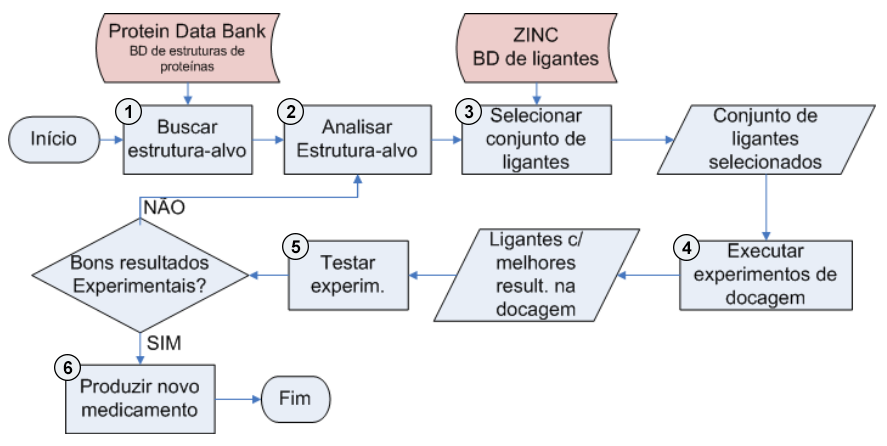
\includegraphics[width=14cm]{images/rdd_workflow.png}
	\label{fig:rddworkflow}
	\caption{\emph{Workflow} do processo de planejamento racional de fármacos assistido por computador \cite{kar11}}
\end{figure}


\begin{enumerate}
  \item O primeiro passo é definir um receptor (normalmente uma proteína) \cite{dre00} e analisar computacionalmente sua estrutura 3D. A estrutura da proteína é determinada por cristalografia por difração de raios X ou ressonância magnética nuclear \cite{far99}, sendo as informações resultantes armazenadas em um banco de dados como o Protein Data Bank - PDB \cite{ber00}. Essa análise tem por objetivo localizar possíveis regiões de ligação onde um ligante pode estabelecer ligações (atividades 1 e 2 do \emph{workflow} da Figura \ref{fig:rddworkflow});
  
  \item Baseado nas prováveis regiões de ligação identificadas no passo anterior, é selecionado um conjunto de possíveis candidatos, chamados ligantes (usualmente pequenas moléculas que podem ser buscadas em Banco de Dados de compostos como o ZINC \cite{irw05}) que podem se ligar a essa região no receptor (atividade 3 \emph{workflow} da Figura \ref{fig:rddworkflow}). As diferentes conformações que determinado ligante pode assumir dentro do sítio de ligação de uma determinada proteína são simuladas por softwares de docking como AutoDock 3.05 \cite{mor98} (atividade 4 do \emph{workflow} da Figura \ref{fig:rddworkflow});
  
  \item Os ligantes que teoricamente obtiveram melhores resultados nas simulções são experimentalmente sintetizados e testados (atividade 5 do \emph{workflow} da Figura \ref{fig:rddworkflow});
  
  \item Baseado nos resultados experimentais, o medicamento é gerado (atividade 6 do \emph{workflow} da Figura \ref{fig:rddworkflow}) ou o processo retorna ao passo 1.
  
\end{enumerate}
  
  Estas quatro etapas descritas por Kuntz \cite{kun92} contemplam apenas as fases de pesquisa e desenvolvimento de um novo medicamento. 
Somente após um longo período de pesquisas e testes in-silico e in-vivo, estabelecendo eficácia e segurança, o novo fármaco é submetido para registro no órgão regulador.

A Tabela \ref{tab:rddtempo} apresenta, de uma forma geral, as etapas e o tempo que contemplam o processo de desenvolvimento de um novo fármaco.

% Please add the following required packages to your document preamble:
% \usepackage{booktabs}
\begin{table}[h]
	\caption{Passos e tempo para desenvolvimento de um novo fármaco \cite{kun92}}
	\label{tab:rddtempo}
	\centering
	\begin{tabular}{@{}lc@{}}
	\toprule
	\multicolumn{1}{c}{\textbf{Passo}}      & \textbf{Tempo (Anos)} \\ \midrule
	Descoberta e geração de um candidato    & 1 - 2                 \\
	Otimização do candidato                 & 1 - 2                 \\
	Ensaios in-vitro e in-vivo              & 1 - 2                 \\
	Testes toxicológicos                    & 1 - 3                 \\
	Testes de segurança em humanos          & 1                     \\
	Testes de eficiência em humanos         & 1 - 2                 \\ \midrule
	\textbf{Tempo total de desenvolvimento} & \textbf{6 - 12}       \\ \bottomrule
	\end{tabular}
\end{table}

O desenvolvimento de fármacos auxiliado por computador (do inglês CADD - Computer-aided drug design) consiste na utilização de recursos, ferramentas e técnicas computacionais contribui de forma significativa para as etapas de desenvolvimento de um fármaco.  Diferentes estágios deste processo podem ser beneficiados pelo uso da computação, podendo ser aplicado na identificação da molécula-alvo, planejamento, análise e melhoramento de ligantes.

As indústrias farmacêuticas aderiram ao uso da bioinformática por se tratar de um método que apresenta um menor custo financeiro, se comparado com os testes tradicionais em laboratórios \cite{art08}. 


\section{Dinâmica Molecular}

O advento da utilização de recursos computacionais aplicado às áreas medicinais e biológicas têm proporcionado o avanço de técnicas e uso de ferramentas que contribuem de forma expressiva para o planejamento racional de fármacos.

A Dinâmica Molecular (DM) é uma técnica de simulação computacional, fundamentada nos princípios da Mecânica Clássica, que possibilita o estudo do comportamento dinâmico microscópico de um sistema molecular, em diferentes intervalos de tempo \cite{nam08}. 

A simulação por DM fornece informações dos átomos individuais que constituem o sistema molecular, permitindo o cálculo de diversas propriedades (pressão, temperatura, volume, energia livre, etc) e análise do potencial de interação dos ligantes na estrutura e estabilidade das proteínas \cite{kar11}.

De acordo com Lesk \cite{art08}, as interações entre os átomos em uma molécula podem ser classificadas de duas maneiras:

\begin{quote}
	(a) Ligações químicas primárias - interações fortes entre átomos que estão localizados bem próximos no espaço. São consideradas interações fixas pois são consistentes em um grande número de conformações, não sendo desfeitas ou alteradas quando a conformação de uma proteína muda. 

	(b) Interações mais fracas que dependem da conformação, podem ser significativas em algumas conformações e não em outras - elas afetam conjuntos de átomos que são aproximados devido a diferentes padrões de enovelamento da cadeia.
\end{quote}

A conformação de uma proteína pode ser especificada pela lista de átomos na estrutura, por suas coordenadas e pelo conjunto de ligações químicas entre eles. A avaliação de uma conformação é feita através do cálculo de conjuntos de potenciais de energia, estes cálculos são computacionalmente complexos e intensivos, mas com a evolução rápida da capacidade de processamento dos computadores esta técnica é beneficiada diretamente \cite{art08}.

A simulação por DM se mostra um método versátil e acessível, sendo considerada a melhor técnica para geração de um conjunto de conformações de um receptor \cite{kar11}. Devido à isso, os dados dos conjuntos de conformações dos receptores utilizados neste trabalho foram gerados utilizando a DM.


\section{Docagem Molecular}

A Docagem Molecular é considerada um dos principais processo do CADD, e é através dela que são produzidos os dados detalhados sobre a interação entre receptores e seus ligantes \cite{LEN96}. 

No processo de Docagem Molecular, algoritmos de docagem são executados para testar e analisar virtualmente a interação entre um ligante e um receptor, estes algoritmos geram um grande número de interações, onde em todas elas, o ligante é testado em diferentes orientações e conformações dentro do sítio de ligação do receptor, de modo a formar um complexo estável. 
Usualmente o receptor é uma proteína ou uma molécula de ácido nucléico, e o ligante pode ser uma pequena molécula ou até mesmo outra proteína. A Figura \ref{fig:docking} \cite{ALE13} ilustra cada um destes elementos e apresenta como é feita a interação entre eles.

\begin{figure}[h]
	\center
	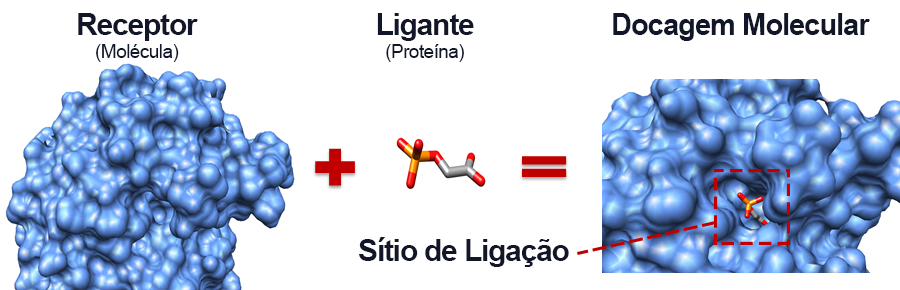
\includegraphics[width=14cm]{images/docking.png}
	\label{fig:docking}
	\caption{Representação do processo de docagem molecular em três dimensões (3D) entre uma proteína como receptor e uma molécula como ligante, na qual se estabelece uma interação entre eles no sítio de ligação do receptor \cite{ALE13}.}
\end{figure}

Diversas interações devem ser testadas para que seja identificado o melhor encaixe do ligante no sítio de ligação do receptor, ou então, a região ou o sítio de ligação deve ser previamente conhecido. Um dos critérios utilizados para avaliar as interações é pelo cálculo da energia livre de ligação (do inglês \emph{FEB - Free Energy of Binding}). Quanto mais negativo for o valor resultante, melhor é a ligação estabelecida \cite{kar07}. A Figura \ref{fig:TCLdocking} \cite{REN13} ilustra o processo de docagem em três dimensões, a posição inicial da molécula do ligante TCL no sítio de ligação da molécula InhA e a posição do ligante TCL após a simulação de docagem molecular.

\begin{figure}[h]
	\center
	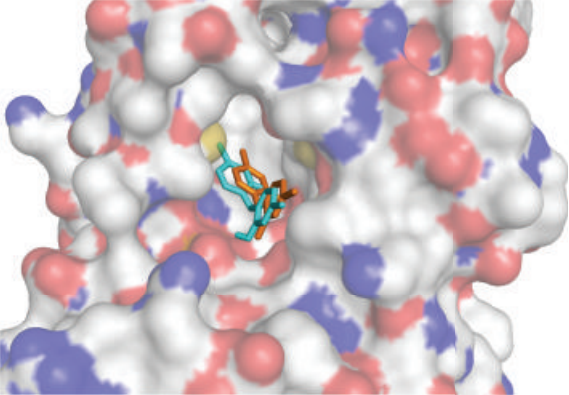
\includegraphics[width=14cm]{images/TCLdocking.png}
	\label{fig:TCLdocking}
	\caption{Representação da superfície molecular do sítio de ligação da enzima receptora InhA na estrutura de cristal. O ligante TCL é  representado na forma de palitos. A conformação inicial do ligante TCL aparece em cor laranja, e a conformação final após uma simulação de docagem molecular é representada em ciano \cite{REN13}.}
\end{figure}

As primeiras abordagens envolvendo a docagem entre proteínas e ligantes consideravam ambos elementos como sendo corpos rígidos. O modelo conhecido como "chave e fechadura" (do inglês \emph{lock-and-key}, proposto por Emil Fisher em 1894, prevê um encaixe perfeito do ligante no sítio de ligação do receptor, tal como uma chave encaixa em sua fechadura correspondente \cite{kar07}. 

No entanto, ambos proteína e ligante são moléculas flexíveis. Desta forma, o modelo histórico de "chave e fechadura" deu seu lugar à novas teorias, as quais passaram a considerar totalmente ou parcialmente a flexibilidade do ligante e do receptor \cite{SOU06}.

Atualmente um dos maiores desafios na área de docagem molecular é conseguir manipular, de forma eficience, a flexibilidade do receptor da proteína. A eficiência da busca pela melhor conformação é determinada pelo número de graus de liberdade  \cite{SOU06}.


Os esforços inicial envolvendo a docagem de protínas e ligantes 


A complexidade aumenta quando, neste processo, são considerados fatores externos, como por exemplo, a flexibilidade do ligante.


\section{Modelagem OLAP}
	Explicação didática sobre o modelo olap para o professor osmar
	Cubos de dados  